\documentclass[10pt,a4paper]{article}

% ---------------------------------------------------------------- packages
\usepackage[T1]{fontenc}
\usepackage[utf8]{inputenc}
\usepackage{lmodern}
\usepackage{microtype}
\usepackage[a4paper,top=2.2cm,bottom=2.4cm,left=2.3cm,right=2.3cm]{geometry}
\usepackage{graphicx}
\usepackage{booktabs,tabularx,array}
\usepackage{caption,subcaption}
\usepackage{titlesec}
\usepackage{enumitem}
\usepackage{float}
\usepackage{longtable}
\usepackage{needspace}
\usepackage{listings}
\usepackage{fancyhdr}
\usepackage{tikz}
\usetikzlibrary{arrows.meta,positioning,fit,calc}
\usepackage[hidelinks,pdftitle={Koto Pai: Final Project Report},
            pdfauthor={Rafsan Riasat, Adib Raian, Utsa Roy}]{hyperref}
\urlstyle{same}

\graphicspath{{../assets/screenshots/}}

% ---------------------------------------------------------------- layout
\setlength{\parindent}{0pt}
\setlength{\parskip}{0.45em}
\linespread{1.0}
\raggedbottom
\setlength{\emergencystretch}{3em}
\setlist{nosep,leftmargin=1.4em,itemsep=2pt,topsep=2pt}

% footer: page number only, no header
\pagestyle{fancy}
\fancyhf{}
\fancyfoot[C]{\thepage}
\renewcommand{\headrulewidth}{0pt}
\renewcommand{\footrulewidth}{0pt}

\titleformat{\section}{\Large\bfseries}{\thesection}{0.7em}{}
\titleformat{\subsection}{\large\bfseries}{\thesubsection}{0.6em}{}
\titleformat{\subsubsection}{\normalsize\bfseries\itshape}{}{0em}{}
\titlespacing*{\section}{0pt}{1.6em}{0.6em}
\titlespacing*{\subsection}{0pt}{1.1em}{0.4em}
\titlespacing*{\subsubsection}{0pt}{0.8em}{0.2em}

\captionsetup{font=small,labelfont=bf,skip=5pt}
\captionsetup[subfigure]{font=footnotesize,skip=3pt}
\captionsetup[table]{skip=4pt}
\captionsetup[longtable]{skip=4pt}

\renewcommand{\arraystretch}{1.18}
\newcolumntype{Y}{>{\raggedright\arraybackslash}X}
\newcommand{\code}[1]{\texttt{#1}}

% framed, colour screenshots
\newcommand{\shot}[2]{{\setlength{\fboxsep}{0pt}\setlength{\fboxrule}{0.4pt}%
  \fbox{\includegraphics[width=\dimexpr#1\linewidth-0.8pt\relax]{#2}}}}

% monochrome listings
\lstset{basicstyle=\ttfamily\footnotesize,keywordstyle=\bfseries,commentstyle=\itshape,
  stringstyle=\ttfamily,frame=tb,framerule=0.4pt,
  breaklines=true,columns=fullflexible,keepspaces=true,xleftmargin=0.6em,xrightmargin=0.6em,
  aboveskip=0.6em,belowskip=0.4em,showstringspaces=false}

% tikz styles shared by the diagrams
\tikzset{
  box/.style={draw,rounded corners=2pt,align=center,inner sep=4pt,font=\footnotesize},
  tbl/.style={draw,align=center,inner sep=3pt,font=\scriptsize,minimum width=2.8cm,minimum height=9mm},
  ev/.style={->,dashed,>=Stealth},
  fk/.style={-,thin},
  idref/.style={-,thin,dashed},
}

\begin{document}

% ================================================================ title page
\begin{titlepage}
\centering
\vspace*{3.2cm}
{\large CSE 3220}\\[6pt]
{\large Software Engineering and Project Management Laboratory}\\[6pt]
{\large Final Project}\\[3cm]
{\fontsize{40}{46}\selectfont\bfseries Koto Pai?}
\vfill
{\Large Submitted by}\\[16pt]
\renewcommand{\arraystretch}{1.6}
\begin{tabular}{lr}
{\Large Rafsan Riasat} & {\Large 2207006} \\
{\Large Adib Raian}    & {\Large 2207020} \\
{\Large Utsa Roy}      & {\Large 2207027} \\
\end{tabular}
\vfill
{\large December 2026}
\vspace*{1.2cm}
\end{titlepage}

% ================================================================ 1 introduction
\section{Introduction}

Friends who share meals, trips and bills tend to remember who paid but not who consumed what. Settling up by memory
causes arguments, and doing it with a calculator loses small amounts: dividing 100.00 among three people as three
rounded shares gives 99.99, and one poisha disappears.

\textbf{Koto Pai?} (Bengali for ``how much do I get?'') is a web application that records an outing item by item,
works out each person's exact position, turns it into debts, and lets people settle, dispute or reroute those debts
with a full history. It was built by a team of three as the final project of the Software Engineering and Project
Management Laboratory, with the course requirements treated as design constraints from the first day: modular
design and recognised patterns, role-based access control, a REST API, automated unit and integration tests in a
pipeline, containers, a public deployment, and monitoring.

\subsection{A worked example}

The whole design is driven by one scenario, \emph{burger night}. Four items are bought: a burger (Tk 200, Rafsan), a
pizza (Tk 500, Tanvir), a cold coffee (Tk 200, Nabila) and a large pizza (Tk 1000, shared 50\%/30\%/20\%). The bill is
Tk 1900; Rafsan paid Tk 1400, Tanvir Tk 500 and Nabila nothing.

\begin{center}
\small
\begin{tabular}{lrrr}
\toprule
 & Consumed (Tk) & Paid (Tk) & Net (Tk) \\
\midrule
Rafsan & 700 & 1400 & +700 \\
Tanvir & 800 & 500 & $-300$ \\
Nabila & 400 & 0 & $-400$ \\
\bottomrule
\end{tabular}
\end{center}

The nets sum to zero, so exactly two debts are generated: Tanvir owes Rafsan Tk 300 and Nabila owes Rafsan Tk 400.
This scenario is a golden test in the calculation engine: if any change shifts a single poisha, the build fails.

\subsection{Money rules}

Amounts are \code{BigDecimal} with scale 2 and never \code{double}; rounding is HALF\_EVEN; calculations run in whole
poisha; input with more than two decimals is rejected rather than silently rounded.

\subsection{Technology}

\begin{table}[H]
\centering\small
\caption{Technology stack.}
\begin{tabularx}{\textwidth}{@{}lY@{}}
\toprule
Concern & Technology \\
\midrule
Language, build & Java 17 source level (Java 21 in CI and Docker), Maven wrapper \\
Framework & Spring Boot 4.1, Spring MVC, Spring Data JPA with Hibernate 7, Bean Validation \\
User interface & Thymeleaf with one layout fragment, hand-written CSS, plain JavaScript for the wizard \\
Security & Spring Security: form login, BCrypt, CSRF, role-based access, method security \\
Database & PostgreSQL 16 (Compose), Neon PostgreSQL (live), H2 for tests and offline runs \\
Testing & JUnit 5, Mockito, AssertJ, MockMvc, Spring Security Test, JaCoCo \\
Delivery & Docker (multi-stage), Docker Compose, GitHub Actions, Render \\
Operations & Spring Boot Actuator, Micrometer, Prometheus, Grafana (local and Grafana Cloud) \\
\bottomrule
\end{tabularx}
\end{table}

% ================================================================ 2 features
\section{Features}

\subsection{Accounts, friends and the dashboard}

Users register (with a confirm-password check), log in with their user ID or e-mail, and edit a profile. Friends are
added by public user ID through requests that can be accepted, rejected or removed. The dashboard shows the net
balance, per-friend balances and active outings at a glance (Figure~\ref{fig:dashboard}).

\begin{figure}[t]
\centering
\shot{0.72}{dashboard.png}
\caption{Dashboard: net balance, balances per friend and active outings.}
\label{fig:dashboard}
\end{figure}

\subsection{Outings and the live split preview}

An outing moves through \code{DRAFT}, \code{ACTIVE} and \code{SETTLED} (or \code{CANCELLED}). The creator adds
participants, items and who paid. Each item is split \emph{personally}, \emph{equally} or \emph{by percentage}. People
without accounts take part as \emph{guests}: they belong to the creator, who stands in for them when debts are
generated.

The wizard saves each step into the draft outing and calls \code{POST /api/outings/preview} as the user types. The
preview runs the \emph{same engine} that runs on submit, so the numbers on screen are the numbers that will be stored,
and every problem is listed at once instead of one error per click (Figure~\ref{fig:wizard}).

\begin{figure}[t]
\centering
\shot{0.72}{wizard-live-preview.png}
\caption{Outing wizard with a live preview that confirms ``Everything adds up''.}
\label{fig:wizard}
\end{figure}

\subsection{The split engine}

The engine is plain Java with no Spring and no JPA, built as a pipeline (Figure~\ref{fig:pipeline}). The
\emph{largest remainder} method gives every share its whole poisha and hands the leftovers to the largest fractions,
so shares always sum to the original amount. Seven validation rules, one class each, collect all problems: at least
one participant, a non-empty bill, known participants, a present guest owner, a consumer for every item, shares that
sum to 100\%, and \textbf{paid equals the bill}. A guest's net is folded into the owner's net, so debts only ever
exist between real users.

\begin{figure}[h]
\centering
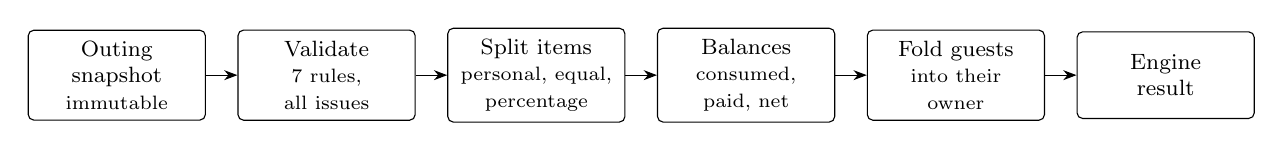
\begin{tikzpicture}[node distance=4mm,>=Stealth,
  pstep/.style={box,minimum width=2.25cm,minimum height=11mm}]
\node[pstep] (a) {Outing\\snapshot\\\scriptsize immutable};
\node[pstep,right=of a] (b) {Validate\\\scriptsize 7 rules,\\\scriptsize all issues};
\node[pstep,right=of b] (c) {Split items\\\scriptsize personal, equal,\\\scriptsize percentage};
\node[pstep,right=of c] (d) {Balances\\\scriptsize consumed,\\\scriptsize paid, net};
\node[pstep,right=of d] (e) {Fold guests\\\scriptsize into their\\\scriptsize owner};
\node[pstep,right=of e] (f) {Engine\\result};
\foreach \x/\y in {a/b,b/c,c/d,d/e,e/f} \draw[->] (\x) -- (\y);
\end{tikzpicture}
\caption{The split engine pipeline. Calculation is deterministic and independent of the framework.}
\label{fig:pipeline}
\end{figure}

\subsection{Ledger and settlement}

When an outing is submitted, the ledger turns the engine's nets into debts in the \emph{same database transaction}.
The debtor records a payment, the creditor confirms it, and partial payments are supported. A disputed debt stops
counting towards balances until resolved. \emph{Delegation} (``skip a step'') lets a middleman settle A$\rightarrow$C
directly when A owes B and B owes C, between mutual friends and reversibly. A greedy simplifier proposes at most
$n-1$ transfers, a guest's owner settles the guest's debts, and optimistic locking guarantees that two simultaneous
Tk 60 payments against a Tk 100 debt result in exactly one success with Tk 40 remaining
(Figure~\ref{fig:ledger}).

\begin{figure}[t]
\centering
\begin{subfigure}[t]{0.485\textwidth}\centering\shot{1}{balances.png}\caption{Balances per friend}\end{subfigure}\hfill
\begin{subfigure}[t]{0.485\textwidth}\centering\shot{1}{settle-up.png}\caption{Settle up: payments, disputes, delegation}\end{subfigure}
\caption{Ledger and settlement pages.}
\label{fig:ledger}
\end{figure}

\subsection{Notifications and activity}

A notification bell and page, and an activity timeline with per-friend history and filters, are driven by
\emph{domain events}: they react to what happened in the outing and ledger modules without those modules knowing they
exist (Figure~\ref{fig:social}).

\begin{figure}[t]
\centering
\begin{subfigure}[t]{0.485\textwidth}\centering\shot{1}{friends.png}\caption{Friends}\end{subfigure}\hfill
\begin{subfigure}[t]{0.485\textwidth}\centering\shot{1}{activity.png}\caption{Activity timeline with filters}\end{subfigure}
\caption{Friends and activity.}
\label{fig:social}
\end{figure}

\subsection{Administration and access control}

There are two roles, \code{USER} and \code{ADMIN}. The Admin Console shows platform statistics (users, outings,
friendships, notifications, settled volume), lists every user with a \textbf{search} by name, handle or e-mail, and
changes roles; the system refuses to demote the last administrator. The administrator is a real account named in
configuration, not a demo account with a published password. Anyone else opening an admin URL receives a friendly 403
page (Figure~\ref{fig:admin}). Admins deliberately cannot read anyone's outings or debts: the console shows aggregates,
not private financial data.

\begin{figure}[t]
\centering
\begin{subfigure}[t]{0.485\textwidth}\centering\shot{1}{admin.png}\caption{Admin Console (\code{ROLE\_ADMIN}) with user search}\end{subfigure}\hfill
\begin{subfigure}[t]{0.485\textwidth}\centering\shot{1}{error-403.png}\caption{A normal user opening \code{/admin}}\end{subfigure}
\caption{Administration and the 403 page.}
\label{fig:admin}
\end{figure}

\subsection{Responsive on every screen}

One layout adapts from a desktop sidebar to a tablet to a phone with a bottom tab bar (Figure~\ref{fig:mobile}).
Signed-out visitors get a public layout without application navigation.

\begin{figure}[t]
\centering
\shot{0.225}{mobile-dashboard.png}\hspace{0.012\textwidth}\shot{0.225}{mobile-outing.png}\hspace{0.012\textwidth}\shot{0.225}{mobile-wizard.png}\hspace{0.012\textwidth}\shot{0.225}{mobile-settle.png}
\caption{Dashboard, outing detail, wizard and settle-up on a phone.}
\label{fig:mobile}
\end{figure}

% ================================================================ 3 software design
\section{Software design}

\subsection{Architecture: a modular monolith}

The system is one deployable with several feature packages and strict boundaries. Modules cooperate through
\emph{services, ports and events}, so any of them could later become its own service. The packages under
\code{com.kotopai} are \code{common}, \code{auth}, \code{user}, \code{friend}, \code{notification}, \code{admin},
\code{outing} (containing the pure-Java \code{engine}), \code{ledger}, \code{activity} and \code{home}: more than 200
production classes and about 100 test classes. Inside a package a request flows controller (pages) or API (REST),
then service or facade, then repository, then domain, with DTOs at the edges. Open-session-in-view is off on purpose,
so a lazy-loading surprise cannot happen in a template.

\begin{figure}[t]
\centering
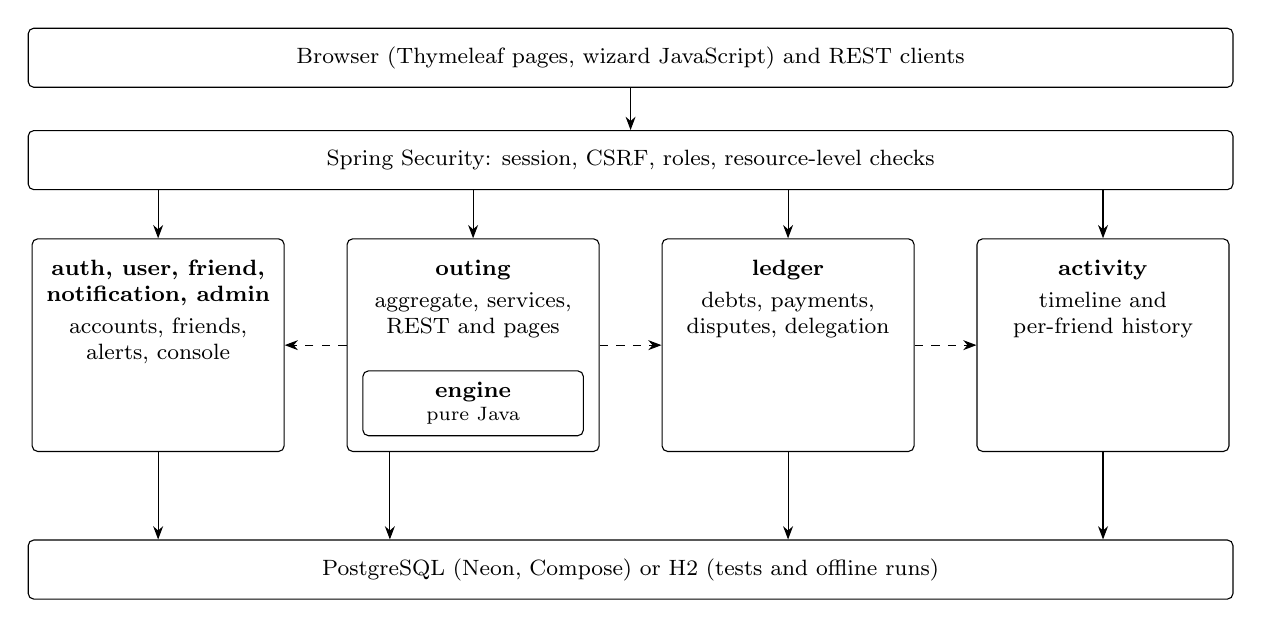
\begin{tikzpicture}[>=Stealth,
  wide/.style={box,minimum width=15.3cm,minimum height=7.5mm},
  mod/.style={box,minimum width=3.2cm,minimum height=27mm}]
\node[wide] (ui) at (0,6.2) {Browser (Thymeleaf pages, wizard JavaScript) and REST clients};
\node[wide] (sec) at (0,4.9) {Spring Security: session, CSRF, roles, resource-level checks};
\node[mod] (acc) at (-6,2.55) {};
\node[mod] (out) at (-2,2.55) {};
\node[mod] (led) at (2,2.55) {};
\node[mod] (act) at (6,2.55) {};
\node[align=center,font=\footnotesize,anchor=north] at ([yshift=-1.5mm]acc.north)
  {\textbf{auth, user, friend,}\\\textbf{notification, admin}\\[2pt]accounts, friends,\\alerts, console};
\node[align=center,font=\footnotesize,anchor=north] at ([yshift=-1.5mm]out.north)
  {\textbf{outing}\\[2pt]aggregate, services,\\REST and pages};
\node[align=center,font=\footnotesize,anchor=north] at ([yshift=-1.5mm]led.north)
  {\textbf{ledger}\\[2pt]debts, payments,\\disputes, delegation};
\node[align=center,font=\footnotesize,anchor=north] at ([yshift=-1.5mm]act.north)
  {\textbf{activity}\\[2pt]timeline and\\per-friend history};
\node[box,minimum width=2.8cm,minimum height=8mm,anchor=south] (eng) at ([yshift=2mm]out.south)
  {\textbf{engine}\\[-1pt]\scriptsize pure Java};
\node[wide] (db) at (0,-0.3) {PostgreSQL (Neon, Compose) or H2 (tests and offline runs)};
\draw[->] (ui) -- (sec);
\foreach \m in {acc,out,led,act} {\draw[->] (sec.south -| \m.north) -- (\m.north);}
\foreach \m in {acc,led,act} {\draw[->] (\m.south) -- (\m.south |- db.north);}
\draw[->] ([xshift=0.55cm]out.south west) -- ([xshift=0.55cm]out.south west |- db.north);
\draw[ev] (out.west) -- (acc.east);
\draw[ev] (out.east) -- (led.west);
\draw[ev] (led.east) -- (act.west);
\end{tikzpicture}
\caption{Module architecture. Solid arrows are calls, dashed arrows are domain events.}
\label{fig:arch}
\end{figure}

The boundary rules, and how honestly they hold:

\begin{itemize}
\item The engine imports no Spring and no JPA; this is enforced by structure, with zero framework imports under
  \code{outing/engine}.
\item Outing, ledger and activity never touch each other's entities or repositories. The ledger asks for outing data
  through the \code{OutingSettlementProvider} port and links by id.
\item Cross-module reactions go through events: outing publishes \code{OutingActivated}, \code{OutingUpdated} and
  \code{OutingCancelled}; the ledger, notifications and activity listen.
\item Outing needs friendship, payment-lock and current-user facts, so it declares its own narrow ports
  (\code{FriendshipChecker}, \code{PaymentLockChecker}, \code{CurrentUserProvider}); adapters in the owning modules
  implement them.
\item \textbf{Exception:} a few read-only views (admin statistics, profile summary, home dashboard, notification text)
  read other modules' repositories directly. They write nothing, and replacing them with query ports is listed as
  future work.
\end{itemize}

\textbf{Submitting an outing} is the heart of the system. The creator posts to \code{/api/outings/\{id\}/submit}; the
service asks the engine to calculate (returning balances or every issue), moves the status from \code{DRAFT} to
\code{ACTIVE}, and publishes \code{OutingActivatedEvent}. The ledger listener generates the debts before the commit
completes, the notification listener reacts to the same event, and the outing and its debts commit together.

\subsection{Design patterns}

Patterns are used where behaviour varies or where a rule must live in exactly one place (Table~\ref{tab:patterns}).

{\small
\begin{longtable}{@{}>{\raggedright\arraybackslash}p{3.1cm}>{\raggedright\arraybackslash}p{4.2cm}>{\raggedright\arraybackslash}p{8.1cm}@{}}
\caption{Design patterns, where they appear and what they solve.}\label{tab:patterns}\\
\toprule
Pattern & Where & Problem it solves \\
\midrule
\endfirsthead
\toprule
Pattern & Where & Problem it solves \\
\midrule
\endhead
\bottomrule
\endfoot
Value Object & \code{Money} & One immutable, scale-2, HALF\_EVEN type; raw \code{BigDecimal} treats 2.0 and 2.00 as different \\
Strategy & \code{SplitStrategy} and three implementations & Split rules vary independently; no growing \code{switch} \\
Template Method & \code{AbstractSplitStrategy} & Common checks run once in a \code{final} method, so no strategy can skip them \\
Factory (registry) & \code{SplitStrategyFactory} & One mapping from split type to strategy; a missing or duplicate one fails at start-up \\
Chain of Responsibility & \code{ValidationRule}, seven rules & Collecting variant: every problem is reported at once \\
Facade & \code{SplitEngine}, \code{OutingApiFacade}, \code{HomePageFacade} & One entry point; callers cannot skip validation \\
Aggregate Root & \code{Outing} & Rules in one place; children saved and deleted with it \\
State & \code{OutingStatus}, \code{DebtStatus} & Legal transitions defined once, not scattered in \code{if} checks \\
Adapter & \code{OutingSnapshotMapper}, \code{EngineSettlementProvider} & Keeps the engine free of JPA and joins modules without importing each other \\
Ports and Adapters & \code{outing/port}, \code{ledger/spi} & Modules build and test before their neighbours exist \\
Observer & Spring events and listeners & Outing does not know the ledger, notifications or timeline exist \\
DTO & \code{outing/api/dto} & Entities never reach JSON; clients cannot over-post fields such as \code{status} \\
Policy object & \code{OutingAccessPolicy} & One place decides who may view or edit; answers 404 to avoid leaking existence \\
\end{longtable}}

\textbf{Strategy, Template Method and Factory} together form the split rules. The base class owns the checks,
subclasses own only the arithmetic, and the factory guarantees that every split type has exactly one strategy. Adding an
``exact amounts'' split means one new strategy and one enum value; forgetting the strategy breaks start-up and a test,
not a customer's bill.

\begin{lstlisting}[language=Java]
public abstract class AbstractSplitStrategy implements SplitStrategy {
    @Override
    public final Map<ParticipantRef, Money> split(ItemLine item) {
        // checks every strategy needs: right type, a consumer, no duplicates
        return Collections.unmodifiableMap(doSplit(item));   // strategy-specific part
    }
    protected abstract Map<ParticipantRef, Money> doSplit(ItemLine item);
}
\end{lstlisting}

\textbf{Observer with ports} keeps modules apart: the outing service publishes an event and the ledger reacts. The
\code{BEFORE\_COMMIT} phase is deliberate. The first version listened \code{AFTER\_COMMIT}, and an integration test
caught an active outing with zero debts, because writes made after the commit were silently lost.

\begin{lstlisting}[language=Java]
@TransactionalEventListener(phase = TransactionPhase.BEFORE_COMMIT,
                            fallbackExecution = true)
public void onOutingActivated(OutingActivatedEvent event) {
    debts.generateDebts(event.outingId());
}
\end{lstlisting}

\textbf{State.} Each status owns its legal transitions; anything else throws an exception that the API maps to
\code{409} (Figure~\ref{fig:states}).

\begin{figure}[t]
\centering
\begin{minipage}[c]{0.44\textwidth}\centering
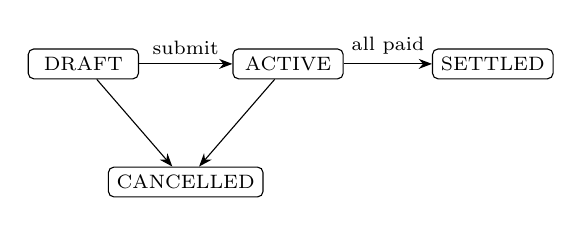
\begin{tikzpicture}[>=Stealth,font=\scriptsize,
  st/.style={draw,rounded corners=2pt,inner sep=3pt,minimum width=1.4cm,align=center}]
\node[st] (d) at (0.4,1.3) {DRAFT};
\node[st] (a) at (3.0,1.3) {ACTIVE};
\node[st] (s) at (5.6,1.3) {SETTLED};
\node[st] (c) at (1.7,-0.2) {CANCELLED};
\draw[->] (d) -- node[above] {submit} (a);
\draw[->] (a) -- node[above] {all paid} (s);
\draw[->] (d) -- (c);
\draw[->] (a) -- (c);
\end{tikzpicture}\\[4pt]
{\footnotesize Outing: cancelling is allowed from DRAFT and ACTIVE.}
\end{minipage}\hfill
\begin{minipage}[c]{0.54\textwidth}\centering
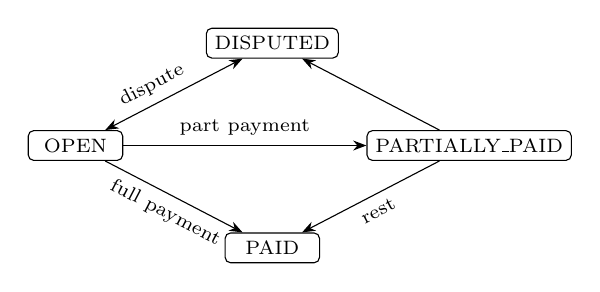
\begin{tikzpicture}[>=Stealth,font=\scriptsize,
  st/.style={draw,rounded corners=2pt,inner sep=3pt,minimum width=1.2cm,align=center}]
\node[st] (x) at (3.5,2.5) {DISPUTED};
\node[st] (o) at (1.0,1.2) {OPEN};
\node[st] (p) at (6.0,1.2) {PARTIALLY\_PAID};
\node[st] (g) at (3.5,-0.1) {PAID};
\draw[->] (o) -- node[above] {part payment} (p);
\draw[->] (o) -- node[below,sloped] {full payment} (g);
\draw[->] (p) -- node[below,sloped] {rest} (g);
\draw[<->] (o) -- node[above,sloped,pos=0.4] {dispute} (x);
\draw[->] (p) -- (x);
\end{tikzpicture}\\[4pt]
{\footnotesize Debt: resolving a dispute returns it to OPEN; VOID from any state when the outing is cancelled.}
\end{minipage}
\caption{State machines of an outing (left) and of a debt (right).}
\label{fig:states}
\end{figure}

\subsection{Design principles}

{\small
\begin{longtable}{@{}>{\raggedright\arraybackslash}p{3.6cm}>{\raggedright\arraybackslash}p{12.2cm}@{}}
\caption{Design principles applied.}\\
\toprule
Principle & Where it is visible \\
\midrule
\endfirsthead
\toprule
Principle & Where it is visible \\
\midrule
\endhead
\bottomrule
\endfoot
Single Responsibility & One validation rule per class; thin controller, facade, service; \code{PersonNames} only resolves names \\
Open/Closed & New split type is a new strategy; new rule is a new class; a new reaction to an outing event is a new listener \\
Liskov Substitution & Every strategy honours the template contract; the calculator depends only on the interface \\
Interface Segregation & Narrow ports (\code{areFriends}, \code{hasRecordedPayments}) instead of whole services \\
Dependency Inversion & Outing depends on its own ports; the engine depends on nothing \\
Fail fast & Factory completeness check, \code{Money} rejects three decimals, health probes at start-up \\
Least privilege & Checks in services \emph{and} URL rules; separate metrics chain; non-root container; secrets from the environment \\
\end{longtable}}

\subsection{Design decisions}

Every decision records the alternative and the reason. The ten that shaped the architecture are listed here.

{\small
\begin{longtable}{@{}p{0.9cm}>{\raggedright\arraybackslash}p{4.4cm}>{\raggedright\arraybackslash}p{3.4cm}>{\raggedright\arraybackslash}p{6.4cm}@{}}
\caption{Key design decisions (numbering follows the project's decision log).}\\
\toprule
\# & Decision & Over & Because \\
\midrule
\endfirsthead
\toprule
\# & Decision & Over & Because \\
\midrule
\endhead
\bottomrule
\endfoot
D1 & Pure-Java calculation engine & A Spring service on entities & Fast, deterministic tests; reused by preview, submit and ledger \\
D2 & Largest-remainder allocation in poisha & Rounding each share & $100/3$ would lose a poisha \\
D3 & Validation collects all errors & Fail on the first & The wizard shows every problem at once \\
D16 & Debts generated \code{BEFORE\_COMMIT} & \code{AFTER\_COMMIT} & Writes after the commit were lost \\
D5 & Wizard saves each step into the draft & HTTP session state & Survives refresh; simpler to test \\
D6 & Ports with stubs between modules & Waiting for teammates & Parallel work, clean seams \\
D17 & Session login, CSRF on, \code{/api} returns 401 & JWT & One model for pages and API \\
D30 & Cross-module links are ids & \code{@ManyToOne} everywhere & Modules stay independent \\
D18 & Render (Docker) and Neon & Railway, Fly.io, Koyeb & Free tiers, reuses the Dockerfile, separate managed database \\
D21 & \code{/actuator/prometheus} behind Basic auth on its own chain & Public, or form login & Prometheus cannot fill a login form; closed by default \\
\end{longtable}}

% ================================================================ 4 data model
\section{Data model}

The schema has 14 tables: \code{users}, \code{friendships}, \code{guests}, \code{outings}, \code{outing\_participants},
\code{items}, \code{item\_shares}, \code{contributions}, \code{debts}, \code{payments}, \code{delegations},
\code{guest\_debts}, \code{notifications} and \code{activity\_events} (Figure~\ref{fig:er}).

\begin{figure}[t]
\centering
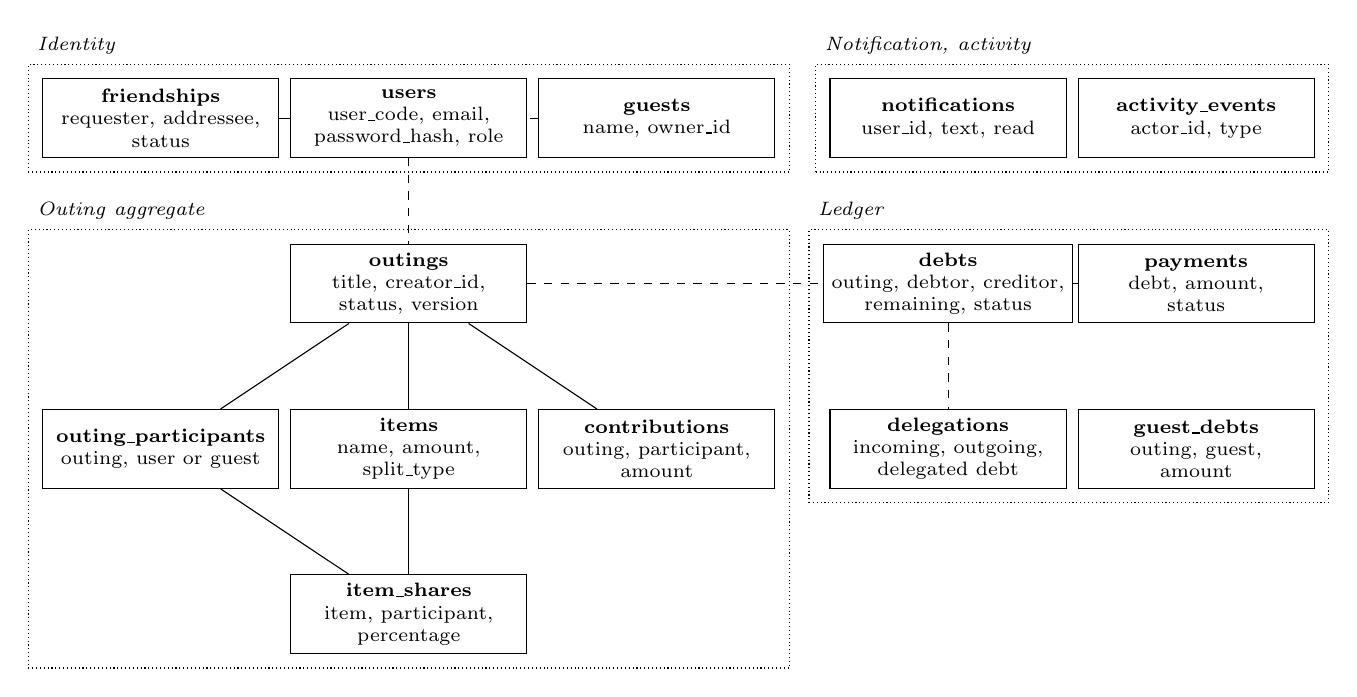
\begin{tikzpicture}[>=Stealth,tbl/.append style={minimum width=3.0cm,minimum height=10mm}]
\node[tbl] (fr) at (-6.55,0) {\textbf{friendships}\\requester, addressee,\\status};
\node[tbl] (us) at (-3.4,0) {\textbf{users}\\user\_code, email,\\password\_hash, role};
\node[tbl] (gu) at (-0.25,0) {\textbf{guests}\\name, owner\_id};
\node[tbl] (ou) at (-3.4,-2.1) {\textbf{outings}\\title, creator\_id,\\status, version};
\node[tbl] (pa) at (-6.55,-4.2) {\textbf{outing\_participants}\\outing, user or guest};
\node[tbl] (it) at (-3.4,-4.2) {\textbf{items}\\name, amount,\\split\_type};
\node[tbl] (co) at (-0.25,-4.2) {\textbf{contributions}\\outing, participant,\\amount};
\node[tbl] (is) at (-3.4,-6.3) {\textbf{item\_shares}\\item, participant,\\percentage};
\node[tbl] (no) at (3.45,0) {\textbf{notifications}\\user\_id, text, read};
\node[tbl] (ac) at (6.6,0) {\textbf{activity\_events}\\actor\_id, type};
\node[tbl] (de) at (3.45,-2.1) {\textbf{debts}\\outing, debtor, creditor,\\remaining, status};
\node[tbl] (pm) at (6.6,-2.1) {\textbf{payments}\\debt, amount,\\status};
\node[tbl] (dl) at (3.45,-4.2) {\textbf{delegations}\\incoming, outgoing,\\delegated debt};
\node[tbl] (gd) at (6.6,-4.2) {\textbf{guest\_debts}\\outing, guest,\\amount};
\draw[fk] (us) -- (fr);
\draw[idref] (gu) -- (us);
\draw[idref] (us) -- (ou);
\draw[fk] (ou) -- (pa);
\draw[fk] (ou) -- (it);
\draw[fk] (ou) -- (co);
\draw[fk] (it) -- (is);
\draw[fk] (pa) -- (is);
\draw[idref] (ou.east) -- (de.west);
\draw[fk] (de) -- (pm);
\draw[idref] (de) -- (dl);
\node[draw,densely dotted,fit=(fr)(us)(gu),inner sep=5pt,
  label={[font=\scriptsize\itshape,anchor=south west]north west:Identity}] {};
\node[draw,densely dotted,fit=(ou)(pa)(it)(co)(is),inner sep=5pt,
  label={[font=\scriptsize\itshape,anchor=south west]north west:Outing aggregate}] {};
\node[draw,densely dotted,fit=(de)(pm)(dl)(gd),inner sep=5pt,
  label={[font=\scriptsize\itshape,anchor=south west]north west:Ledger}] {};
\node[draw,densely dotted,fit=(no)(ac),inner sep=5pt,
  label={[font=\scriptsize\itshape,anchor=south west]north west:Notification, activity}] {};
\end{tikzpicture}
\caption{Entity-relationship overview. Solid lines are JPA relationships inside a module; dashed lines are references
by id between modules. Dotted boxes are module boundaries.}
\label{fig:er}
\end{figure}

\begin{itemize}
\item \textbf{One-to-many with cascade:} \code{Outing} to participants, items and contributions, and \code{Item} to
  shares (\code{cascade = ALL}, \code{orphanRemoval}); children exist only through the aggregate root.
\item \textbf{Many-to-one:} participant to outing and guest, item to outing, share to item and participant, payment to
  debt, friendship to user.
\item \textbf{Many-to-many through a junction entity:} users through \code{Friendship} (carrying its status), items and
  participants through \code{ItemShare} (carrying the percentage), outings and people through
  \code{OutingParticipant}.
\item \textbf{Logical id references with no foreign key:} links between modules, such as \code{Outing.creatorId},
  \code{Debt.outingId}, \code{Debt.debtorId} and \code{Notification.userId} (decision D30). The ledger, notification
  and activity modules never import \code{User} or \code{Outing} entities. The trade-off is explicit: integrity
  \emph{between} modules is enforced in services, and \emph{inside} an aggregate by JPA relationships.
\end{itemize}

Other integrity rules: unique \code{userCode} and e-mail, one friendship per pair, \code{NUMERIC(12,2)} for money, and
optimistic locking (\code{@Version}) on \code{Outing} and \code{Debt}.

% ================================================================ 5 rest api
\section{REST API}

The application exposes \textbf{38 endpoints in 11 controllers}. Authentication is the session cookie from form login,
and every state-changing request needs a CSRF token. Unauthenticated \code{/api} calls return 401, while pages redirect
to the login page. Errors are RFC~9457 problem-details JSON~\cite{rfc9457}: 400 invalid input, 403, 404 (also used for
resources a user may not see, so their existence does not leak), 409 illegal state or conflict, and 422 for an outing
that cannot be calculated yet. The API never accepts a user id from the client; the acting user always comes from the
authenticated principal.

\Needspace{9\baselineskip}
{\small
\begin{longtable}{@{}>{\raggedright\arraybackslash}p{2.1cm}>{\raggedright\arraybackslash}p{6.7cm}>{\raggedright\arraybackslash}p{6.5cm}@{}}
\caption{Endpoints grouped by controller. Server-rendered pages sit beside the API.}\\
\toprule
Area & Endpoints & Access \\
\midrule
\endfirsthead
\toprule
Area & Endpoints & Access \\
\midrule
\endhead
\bottomrule
\endfoot
Auth & \code{POST /api/auth/register} & public \\
Profile & \code{GET, PUT /api/me}; \code{GET /api/users/\{userCode\}} & login \\
Friends & \code{GET /api/friends}; requests: list, send, accept, reject; \code{DELETE /api/friends/\{id\}} & login; addressee answers \\
Guests & \code{GET, POST /api/guests}; \code{DELETE /api/guests/\{id\}} & owner \\
Outings & create, list, read, \code{PUT} (replace), \code{DELETE} (draft), \code{POST /api/outings/preview}, \code{/submit}, \code{/cancel} & creator; participants read once not a draft \\
Ledger & \code{GET /api/ledger}, \code{GET /api/debts} & current user \\
Settlement & record payment, confirm payment, dispute a debt & debtor or creditor; only the creditor confirms \\
Guest debts & \code{GET /api/guest-debts}, settle & guest owner \\
Delegation & suggestions, execute & middleman \\
Notifications & list, unread count, mark read, read all & owner \\
Activity & \code{GET /api/activity} with \code{friendId}, \code{type} filters & current user \\
Admin & \code{GET /api/admin/stats}, \code{GET /api/admin/users?q=}, \code{POST /api/admin/users/\{id\}/role} & \textbf{ROLE\_ADMIN} \\
Operations & \code{/actuator/health} (probes); \code{/actuator/prometheus} & public; HTTP Basic for the scrape account \\
\end{longtable}}

As an example, the live preview takes a draft and returns balances without saving anything. Incomplete input is still a
normal \code{200} with \code{"valid": false} and \emph{every} problem in \code{issues}, for example \code{NO\_ITEMS}
and \code{PAID\_NOT\_EQUAL\_BILL} together.

\begin{lstlisting}
POST /api/outings/preview   (two participants, one Tk 800 item split equally, user 1 paid 800)

{ "valid": true, "issues": [], "billTotal": 800.00, "paidTotal": 800.00,
  "balances": [ { "userId": 1, "consumed": 400.00, "paid": 800.00, "net":  400.00 },
                { "userId": 2, "consumed": 400.00, "paid":   0.00, "net": -400.00 } ] }
\end{lstlisting}

% ================================================================ 6 security
\Needspace{10\baselineskip}
\section{Security}

{\small
\begin{longtable}{@{}>{\raggedright\arraybackslash}p{3.3cm}>{\raggedright\arraybackslash}p{12.2cm}@{}}
\caption{Security measures.}\\
\toprule
Area & What is implemented \\
\midrule
\endfirsthead
\toprule
Area & What is implemented \\
\midrule
\endhead
\bottomrule
\endfoot
Authentication & Form login with a session cookie; passwords hashed with BCrypt (a test proves the stored hash differs from the password) \\
Role-based access & \code{USER} and \code{ADMIN}; \code{/admin/**} and \code{/api/admin/**} require \code{ROLE\_ADMIN}; method security with \code{@PreAuthorize} on the admin service; everything else is authenticated by default \\
Resource-level checks & Outings are visible to the creator and, once submitted, participants (hidden and unknown both return 404); debts only to debtor and creditor; payments confirmed only by the creditor; delegation only by the middleman \\
CSRF & Enabled for every state-changing request; tests prove a POST without a token is rejected \\
Input validation & Bean Validation on every request DTO plus engine rules for business validation \\
Concurrency & \code{@Version} on \code{Debt} and \code{Outing}, proven by a concurrent-payment test \\
Errors & Problem-details handlers and branded error pages with no stack traces or exception names \\
Operations & Non-root container user; secrets only from the environment; the metrics endpoint has its own Basic-auth chain; the administrator comes from configuration, not a demo seed \\
\end{longtable}}

Three vulnerabilities were found and fixed during the project: an early home page showed any user's ledger through a
\code{?userId=} parameter (removed; identity comes only from the principal); a non-public error page caused a
post-login redirect to a raw JSON page; and a health check behind login reported the container healthy while the
application was broken.

% ================================================================ 7 testing
\section{Testing}

The suite has \textbf{760 tests: 658 unit and 102 integration, with no failures}; the requirement was at least 20 and
10. Unit tests (\code{*Test}, run by Surefire) use JUnit 5, Mockito, AssertJ, parameterised tests, \code{@WebMvcTest}
and \code{@DataJpaTest}. Integration tests (\code{*IT}, run by Failsafe) use \code{@SpringBootTest} and MockMvc with the
real security filter chain and H2. Engine line coverage is 100\% with an 80\% gate enforced by JaCoCo in the pipeline.

\begin{itemize}
\item \textbf{Golden-master engine tests:} hand-worked scenarios (burger night, a guest called Rahim) assert exact
  numbers, and 200 seeded random cases prove shares always sum exactly and each lies within one poisha.
\item \textbf{Security matrices:} every ledger and activity route is called anonymously and as an unrelated user;
  outing visibility, CSRF, 401/403/404, admin role checks and the metrics endpoint are covered.
\item \textbf{End-to-end flows:} create, submit, debts, cancel, void; dispute, regenerate, partial and final payment
  to settled; two concurrent payments.
\item \textbf{Admin features:} the bootstrap runner (promote, create, reject a short password, never crash start-up),
  the seed rule that keeps the demo admin off hosted deployments, and the user search through the full stack
  including a check that \code{\%} is matched literally.
\item \textbf{Integration tests found defects unit tests could not:} a missing cascade (data not saved although the
  unit test passed), debts silently lost with \code{AFTER\_COMMIT}, guests that would have been counted twice, and CSRF
  being checked before authentication.
\item \textbf{The pipeline catches regressions:} an intentional \code{BigDecimal.equals} bug turned the unit job red
  and skipped integration, then went green after the \code{compareTo} fix.
\item \textbf{Not covered automatically:} the wizard's JavaScript. It is covered by the API tests it calls and a
  15-minute manual test script.
\end{itemize}

% ================================================================ 8 ci/cd
\section{CI/CD and Git workflow}

Work follows \emph{one task, one branch, one pull request}. Feature branches merge into \code{develop} by pull request
with CI; \code{develop} merges into \code{main} through a release pull request. \code{main} is protected: no direct
pushes, at least one approval and green required checks. Merge commits are used on purpose so the history, including
intentional red commits, stays visible.

\begin{figure}[h]
\centering
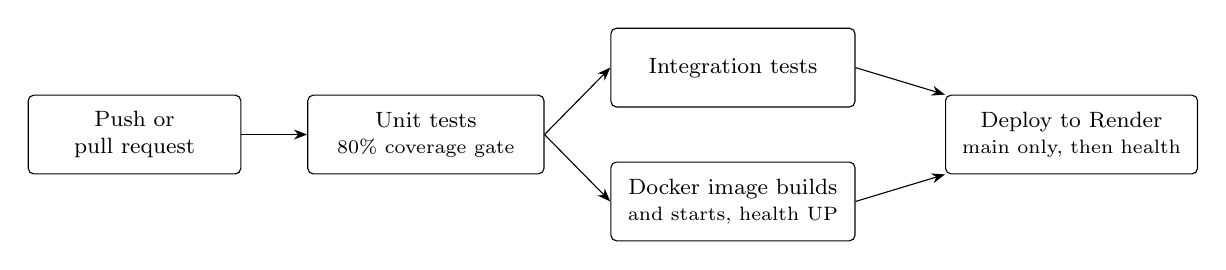
\begin{tikzpicture}[>=Stealth,
  cistep/.style={box,minimum height=10mm,minimum width=2.7cm}]
\node[cistep] (p) at (0,0) {Push or\\pull request};
\node[cistep,minimum width=3cm] (u) at (3.7,0) {Unit tests\\\scriptsize 80\% coverage gate};
\node[cistep,minimum width=3.1cm] (i) at (7.6,0.85) {Integration tests};
\node[cistep,minimum width=3.1cm] (d) at (7.6,-0.85) {Docker image builds\\\scriptsize and starts, health UP};
\node[cistep,minimum width=3.2cm] (r) at (11.9,0) {Deploy to Render\\\scriptsize main only, then health};
\draw[->] (p) -- (u);
\draw[->] (u.east) -- (i.west);
\draw[->] (u.east) -- (d.west);
\draw[->] (i.east) -- (r.north west);
\draw[->] (d.east) -- (r.south west);
\end{tikzpicture}
\caption{The GitHub Actions pipeline (\code{.github/workflows/ci.yml}).}
\label{fig:cicd}
\end{figure}

Superseded runs are cancelled, permissions are limited to \code{contents: read}, and Render's own auto-deploy is turned
\emph{off}, so only this pipeline can release. Deployment calls a Render deploy hook, kept as a repository secret,
for the exact commit and then polls the public health check. The deploy job runs only for pushes to \code{main}, so
on other branches it is skipped by design (Figure~\ref{fig:ci}).

\begin{figure}[t]
\centering
\begin{subfigure}[t]{0.485\textwidth}\centering\shot{1}{ci-pipeline.jpg}\caption{Job graph}\end{subfigure}\hfill
\begin{subfigure}[t]{0.485\textwidth}\centering\shot{1}{merged-pull-requests.jpg}\caption{Merged pull requests}\end{subfigure}
\caption{Continuous integration on GitHub.}
\label{fig:ci}
\end{figure}

% ================================================================ 9 docker, hosting, monitoring
\section{Containers, hosting and monitoring}

\subsection{Docker}

The \code{Dockerfile} has three stages. The \emph{builder} (Maven with Java 21) copies \code{pom.xml} first for layer
caching, resolves dependencies through a Maven Central mirror with retries, and packages the jar without re-running
unit tests, which already run in CI. The \emph{extractor} unpacks the Spring Boot layered jar, so rarely changing
dependencies and often changing application code sit in different layers. The \emph{runner} uses a Java 21 JRE image,
a \textbf{non-root} user, layers copied in order of change frequency, container-aware JVM memory settings, it honours
the \code{PORT} variable, and has a \code{HEALTHCHECK} that requires \code{"status":"UP"}~\cite{docker}.

Docker Compose runs PostgreSQL 16 (with a health check and a persistent volume) and the application, which starts only
once the database is healthy. An optional \code{monitoring} profile adds Prometheus and Grafana, provisioned from
files in the repository.

\subsection{Hosting}

\begin{table}[H]
\centering\small
\caption{Where each part runs.}
\begin{tabularx}{\textwidth}{@{}>{\raggedright\arraybackslash}p{2.6cm}Y@{}}
\toprule
Part & Where and how \\
\midrule
Application & Render~\cite{render}: Docker web service on the free tier, built from the repository \code{Dockerfile}; health check path \code{/actuator/health}; CI triggers releases \\
Database & Neon~\cite{neon}: managed PostgreSQL, SSL required, same region as the service \\
CI/CD & GitHub Actions~\cite{actions} \\
Monitoring & Grafana Cloud~\cite{grafana}, scraping the application once a minute \\
Live URL & \url{https://koto-pai-aatd.onrender.com} (free instances sleep after about 15 minutes idle and need about a minute to wake) \\
\bottomrule
\end{tabularx}
\end{table}

A request to \code{/actuator/health} on the live URL returns \code{"status":"UP"}. Configuration comes entirely from environment variables, with development-only defaults in Compose and no secrets in
the repository. Besides the database and profile settings, \code{KOTOPAI\_ADMIN\_USER\_CODE} names the account that
becomes the administrator: on every start the application promotes that user, or creates the account when an e-mail
and a password are also supplied. The bootstrap is idempotent and never logs the password.

\begin{figure}[t]
\centering
\begin{subfigure}[t]{0.485\textwidth}\centering\shot{1}{render-deploys.jpg}\caption{Render service and deploys}\end{subfigure}\hfill
\begin{subfigure}[t]{0.485\textwidth}\centering\shot{1}{prometheus-targets.png}\caption{Prometheus target page: application UP}\end{subfigure}
\caption{Hosting and metrics scraping: the Render service and its deploys, and the application as a Prometheus target.}
\label{fig:render}
\end{figure}

\subsection{Monitoring}

Spring Boot Actuator exposes \code{/actuator/health} (with liveness and readiness probes) publicly, and keeps other
endpoints behind login. Micrometer publishes metrics to \code{/actuator/prometheus}, protected by HTTP Basic on a
\emph{separate filter chain} and closed entirely when no password is configured; metrics carry the tag
\code{application=kotopai}, and latency histograms give the 50th, 95th and 99th percentiles~\cite{micrometer,prometheus}.

The dashboard \emph{Koto Pai -- Application Overview} has 12 panels, versioned as JSON in the repository: application
status, uptime, requests per second, the 5xx rate, heap, live threads, requests by status, response-time percentiles,
latency by endpoint, JVM memory, the HikariCP connection pool, and CPU. It can be viewed three ways: the local Compose
profile, a laptop-hosted stack pointed at the live site, and a hosted Grafana Cloud dashboard that stays up without
anyone's laptop (Figure~\ref{fig:grafana}). Rate windows are five minutes because Grafana Cloud scrapes once a
minute and \code{rate()} needs two samples. The 5xx tile shows 0 rather than ``No data'' when there are no errors.

\begin{figure}[t]
\centering
\begin{subfigure}[t]{0.485\textwidth}\centering\shot{1}{grafana-cloud-top.jpg}\caption{Status, traffic and latency}\end{subfigure}\hfill
\begin{subfigure}[t]{0.485\textwidth}\centering\shot{1}{grafana-cloud-bottom.jpg}\caption{Endpoints, JVM, connection pool, CPU}\end{subfigure}
\caption{The Grafana Cloud dashboard for the live site.}
\label{fig:grafana}
\end{figure}

% ================================================================ 10 project management
\section{Project management and contributions}

\subsection{Process}

\begin{itemize}
\item \textbf{Incremental delivery:} a written roadmap of numbered tasks, each with a definition of done, delivered in
  short cycles of one to three tasks per day.
\item \textbf{One task, one branch, one pull request,} with unit and integration tests alongside the code, and a
  per-task work log of what was built, which tests ran and which decisions were taken.
\item \textbf{Contracts first:} cross-module interfaces (events, the settlement provider, and the debt, notification and
  friend services) were agreed in an architecture document before parallel work started, so a module could build
  against a port with a stub before its neighbour existed.
\item \textbf{Integration checkpoints:} the three modules were reconciled on \code{develop} on scheduled days, each
  check recording what matched and what had to change.
\item \textbf{Quality gates:} protected \code{main}, required checks, review approval, coverage gate, Docker start-up
  check, and deployment only after everything is green.
\end{itemize}

\subsection{Team and contributions}

Each member owned a vertical slice end to end: service, API, pages and tests.

\begin{table}[H]
\centering\small
\caption{Ownership of the modules.}
\begin{tabularx}{\textwidth}{@{}>{\raggedright\arraybackslash}p{3.0cm}l Y@{}}
\toprule
Member & Roll & Contribution \\
\midrule
Rafsan Riasat & 2207006 & \code{outing} and the split engine, dashboard, demo data, CI pipeline, Docker and deployment hardening, monitoring, UI polish, admin bootstrap and user search \\
Adib Raian & 2207020 & \code{ledger} (debts, payments, disputes, delegation, guest debts, simplifier), \code{activity}, ledger and activity pages \\
Utsa Roy & 2207027 & \code{auth}, \code{user}, \code{friend}, \code{notification}, \code{admin}, \code{common}, base layout, security hardening \\
\bottomrule
\end{tabularx}
\end{table}

\Needspace{12\baselineskip}
\subsection{Timeline}

{\small
\begin{longtable}{@{}>{\raggedright\arraybackslash}p{2.6cm}>{\raggedright\arraybackslash}p{12.9cm}@{}}
\caption{Project timeline.}\\
\toprule
Date (2026) & Milestone \\
\midrule
\endfirsthead
\toprule
Date (2026) & Milestone \\
\midrule
\endhead
\bottomrule
\endfoot
Oct 28--31 & Repository, test tooling, CI pipeline, engine core \\
Nov 5--6 & Ledger phases 0--1; engine complete, entities, lifecycle, adapters \\
Nov 14 & Services, events, REST API, live preview, integration suite; authentication and layout \\
Nov 15--24 & Payments, delegation, friends, profile, notifications, activity; outing pages \\
Nov 25 & Hardening, wizard with live preview, dashboard, demo data \\
Nov 27 & Deployment, monitoring, build fixes, CI deploy job, hosted Grafana \\
Nov 28 & Real administrator through configuration, admin user search, README \\
\end{longtable}}

\Needspace{9\baselineskip}
\subsection{What went wrong, and what it taught}

{\small
\begin{longtable}{@{}>{\raggedright\arraybackslash}p{4.7cm}>{\raggedright\arraybackslash}p{4.2cm}>{\raggedright\arraybackslash}p{6.4cm}@{}}
\caption{Selected problems and lessons.}\\
\toprule
Problem & Cause & Lesson \\
\midrule
\endfirsthead
\toprule
Problem & Cause & Lesson \\
\midrule
\endhead
\bottomrule
\endfoot
Valid \code{100.00} percentages rejected & \code{BigDecimal.equals} compares scale & Use \code{compareTo}; realistic inputs find real bugs \\
Data not saved although the unit test passed & Missing cascade & Integration tests exist for a reason \\
Submit left an active outing with no debts & \code{AFTER\_COMMIT} listener writes were lost & Cross-module tests find contract bugs \\
\end{longtable}}

% ================================================================ 11 limitations
\section{Limitations and future work}

\begin{itemize}
\item Cross-module references are ids rather than foreign keys, and a few read-only views read other modules'
  repositories; small query ports would remove that.
\item The schema is managed by Hibernate \code{ddl-auto=update} rather than Flyway or Liquibase.
\item There is no login rate limiting, password reset or e-mail verification, and the live site keeps public demo
  accounts for users.
\item Only \code{USER} and \code{ADMIN} roles exist, and the admin role is deliberately limited to analytics and role
  management.
\item The free hosting tier sleeps when idle, the application is a single instance with in-memory sessions, and the
  wizard's JavaScript has no automated tests.
\item A second-platform deployment was not done. Ideas for later: an exact-amounts split strategy (the Strategy seam is
  ready), receipts and attachments, recurring outings and push notifications.
\end{itemize}

% ================================================================ 12 conclusion
\section{Conclusion}

Koto Pai turns a familiar social problem into a small system whose core is exact and well tested: a pure calculation
engine, a ledger that records every debt and payment, and a REST API and web interface on top. The project met its
requirements and was run the way a team should work. Contracts were agreed first, every task had its own branch and
pull request, and a pipeline with coverage and start-up gates stood between a change and production. The application is
deployed publicly, monitored with Prometheus and Grafana, and documented. Choosing patterns for a reason (strategy
where behaviour varies, events where modules must stay apart, state where transitions must be legal) kept the code
changeable, and the defects that did occur were found by tests and fixed early. The honest limitations listed above are
the natural next steps.

% ================================================================ references
\Needspace{24\baselineskip}
\begin{thebibliography}{99}\footnotesize
\setlength{\itemsep}{1pt}\setlength{\parskip}{0pt}
\bibitem{springboot} Spring Boot Reference Documentation. \url{https://docs.spring.io/spring-boot/}
\bibitem{springsec} Spring Security Reference. \url{https://docs.spring.io/spring-security/reference/}
\bibitem{hibernate} Hibernate ORM Documentation. \url{https://hibernate.org/orm/documentation/}
\bibitem{thymeleaf} Thymeleaf Documentation. \url{https://www.thymeleaf.org/documentation.html}
\bibitem{postgres} PostgreSQL Documentation. \url{https://www.postgresql.org/docs/}
\bibitem{neon} Neon Documentation (serverless PostgreSQL). \url{https://neon.com/docs}
\bibitem{render} Render Documentation (Docker web services, deploy hooks, health checks). \url{https://render.com/docs}
\bibitem{docker} Docker Documentation (multi-stage builds, Compose). \url{https://docs.docker.com/}
\bibitem{actions} GitHub Actions Documentation. \url{https://docs.github.com/en/actions}
\bibitem{micrometer} Micrometer Documentation. \url{https://docs.micrometer.io/}
\bibitem{prometheus} Prometheus Documentation. \url{https://prometheus.io/docs/}
\bibitem{grafana} Grafana Cloud Documentation. \url{https://grafana.com/docs/grafana-cloud/}
\bibitem{junit} JUnit 5 User Guide, \url{https://junit.org/junit5/docs/current/user-guide/}; Mockito,
  \url{https://site.mockito.org/}; JaCoCo, \url{https://www.jacoco.org/jacoco/trunk/doc/}
\bibitem{rfc9457} M. Nottingham, E. Wilde, S. Dalal, \emph{Problem Details for HTTP APIs}, RFC 9457, IETF, 2023.
  \url{https://www.rfc-editor.org/rfc/rfc9457}
\bibitem{gof} E. Gamma, R. Helm, R. Johnson, J. Vlissides, \emph{Design Patterns: Elements of Reusable Object-Oriented
  Software}, Addison-Wesley, 1994.
\bibitem{martin} R. C. Martin, \emph{Clean Architecture}, Prentice Hall, 2017.
\bibitem{evans} E. Evans, \emph{Domain-Driven Design}, Addison-Wesley, 2003.
\bibitem{cockburn} A. Cockburn, \emph{Hexagonal Architecture (Ports and Adapters)}.
  \url{https://alistair.cockburn.us/hexagonal-architecture/}
\end{thebibliography}

\end{document}
